\section{Applications of Laplace analysis to the Cauchy problem (initial value problem)}

With the above formulas we can '\textit{invert}' the Laplace transform of many functions. That is the say, if we have a function that is the Laplace function of something, there is a lot of case were can we find what is \important{something} is. Note that we will also see the formal definition of the Laplace transform.


\subsection{Ordinary Differential Equations (ODE) with constant coefficients}
\begin{parag}{First order initial value problem}
The first type of equations we will talk about is first order initial value problem. Formally we have:\\
$ $\\
Let $a, y_0 \in \mathbb{R}$ and $f: \mathbb{R}_+ \to \mathbb{R}$ be piecewise continuous. The task is to find a solution $y : \mathbb{R}_+ \to \mathbb{R}$ solving 
\begin{align*} 
	\begin{cases}
		y'\left(t\right) + ay\left(t\right) = f\left(t\right) \mathspace \forall t > 0\\
		y\left(0\right) =  y_0
	\end{cases}
	\end{align*}
	We will address two question
	\begin{itemize}
		\item \important{existence}: whether there is a solution or not (this will be done using Laplace analysis).
		\item \important{uniqueness}: there is a unique solution
	\end{itemize}
	\begin{subparag}{Remark}
	    In general, we will have linear initial value problems (i.e., no non linear dependency on the sought solution $y$ such as $y\left(t\right)^2, y\left(t\right)^3$, etc.). Also, if the number of initial conditions is equal to the order of the equation then the solution is unique. (e.g.,  $y\left(0\right) = y_0$ above)
	\end{subparag}
	\begin{proof}
	Now we will prove the uniqueness of the equation written above. To do so let us have two solutions $y_1, y_2 : \mathbb{R}_+ \to \mathbb{R}$, the goal is to show that they coincide. We will do this by showing that $w\left(t\right) = 0 \forall t \in \mathbb{R}_+$, where $w\left(t\right) =  y_1\left(t\right) - y_2\left(t\right)$.\\
	$ $\\
	First we know that both $y_1$ and $y_2$ satisfy the equation, using that we will try to derive a differential equation for $w$. In this case this is easy as because $w$ solve this differential equation (as this is linear combinations).
	\begin{align*} 
		\begin{cases}
			w'\left(t\right) + a w\left(t\right) &= 0\\
			w\left(0\right) &= 0
		\end{cases}
	\end{align*}
	It is pretty easy to see that $w\left(t\right) = 0$ is a solution, but we also need to prove that it is the \important{only} solution. To do so we will multiply $w$ with $e^{at}$. Then the previous equation gives 
	\begin{align*} 
		\left(e^{at}w\left(t\right)\right)' &= ae^{at}w\left(t\right) + e^{at}w'\left(t\right)\\
			&= ae^{at} w\left(t\right) - ae^{at}w\left(t\right) = 0
	\end{align*}
	Hence $e^{at}w\left(t\right)$ is constant in $t \in \mathbb{R}_+$. And as $e^{at}w\left(t\right) = e^{a0}w\left(0\right) = 0$, this shows that $w\left(t\right) = 0 $ for all $t \in \mathbb{R}_+$.
	\end{proof}
	Now let us proof \important{Existence}
	\begin{proof}
	    To do so we will use the Laplace transform of the differential equation 
		\begin{align*} 
			y'\left(t\right) + ay\left(t\right) = f\left(t\right)
		\end{align*}
		Let us apply Laplace (we will be deliberate on the existence of the Laplace transform here)
		\begin{align*} 
			\mathcal{L}\left[y'\right]\left(z\right) + a\mathcal{L}\left[y\right]\left(z\right) = \mathcal{L}\left[f\right]\left(z\right)
		\end{align*}
		Let us now set $Y =  \mathcal{L}\left[y\right]$ and $F =  \mathcal{L}\left[f\right]$ and using the formula for the Laplace transform of derivative we have:
		\begin{align*} 
			z Y\left(z\right) -\underbrace{y\left(0\right)}_{=  y_0} + a Y\left(z\right) =  F\left(z\right)
		\end{align*}
		By solving this we get 
		\begin{align*} 
			Y\left(z\right) = \frac{F\left(z\right)}{z + a} + \frac{y_0}{z + a}
		\end{align*}
		We use the punchline: '\textit{derivatives transform derivatives equations to algebraic equations}'\\
		$ $\\
		The question we need to answer is, does the right hand side of the above expression is a Laplace transform of something? To do so we can recall that:
		\begin{align*} 
			\frac{1}{z + a} =  \mathcal{L}\left[e^{-at}\right]\left(z\right)
		\end{align*}
		This implies that we get 
		\begin{align*} 
			Y\left(z\right) =  \mathcal{L}\left[e^{-at}\right]\left(z\right)\mathcal{L}\left[f\right]\left(z\right) + y_0 \mathcal{L}\left[e^{-at}\right]\left(z\right)
		\end{align*}
		We can see here that the first part of the right hand side is the Laplace transform of the convolution of $e^{-at}$ with $f\left(t\right)$! This would '\textit{implies}' that 
		\begin{align*} 
			y\left(t\right) = \int_{0}^{t} e^{-a\left(t-s\right)}f\left(s\right)ds + y_0e^{-at}
		\end{align*}
		Indeed one can verify that this is a solution of the differential equation.
	\end{proof}
	
\end{parag}




\begin{parag}{Second order initial value problem}
    	Now let us go into the second order. To do so we will define it as:
		\begin{definition}
			Let $w \in \mathbb{R}_+, a > 0$, and $f: \mathbb{R}_+ \to \mathbb{R}$ as above 
			\begin{align*} 
				\begin{cases}
					y''\left(t\right) + 2ay'\left(t\right) + w^2 y\left(t\right) &=  f\left(t\right) \mathspace \mathspace \forall t > 0\\
					y\left(0\right) &=  y_0\\
					y'\left(0\right) &= v_0
				\end{cases}
			\end{align*}
		\end{definition}
		\begin{subparag}{Remark}
		    This is the equation satisfied by the harmonic oscillator, $f$ is representing a forcing parameter
		\end{subparag}
		As in the first order case we also have uniqueness
		\begin{subparag}{Uniqueness}
		    \begin{proof}
		        Let $y_1, y_2: \mathbb{R}_+ \to \mathbb{R}$ be two solutions of the ODE. Let us set $w\left(t\right) = y_1\left(t\right) - y_2\left(t\right)$. As above we want to show that $w\left(t\right) = 0 \mathspace \mathspace \; \forall t \in \mathbb{R}_+$ by using \important{energy method}.\\
				$ $\\
				To do so, we will subtract in the ODE $y_2$ from $y_1$ this gives us
				\begin{align*} 
					\begin{cases}
						w''\left(t\right) + 2aw'\left(t\right) + \omega^2 w\left(t\right) &= 0 \\
					w\left(0\right) &= 0\\
					w'\left(0\right) &= 0
					\end{cases}
				\end{align*}
				Let us now magically multiply the equation by $w'$:
				\begin{align*} 
						\underbrace{u''u'}_{= \frac{1}{2}\left(\left(u'\right)^2\right)'} + 2a\left(u'\right)^2 + \omega^2 \underbrace{u'u}_{= \frac{1}{2}\left(u^2\right)'} = 0\\
																																										\implies \left(\frac{1}{2}\left(w'\right)^2\right)' + 2a \left(w'\right)^2 + \left(\frac{1}{2}\omega^2 w^2\right)'
				\end{align*}
				And as we can see, the left part here is the kinetic energy and the right part is the potential energy, this is why this is called the energy method.\\
				Then this implied that:
				\begin{align*} 
					\left(\frac{1}{2}\left(u'\right)^2  + \frac{1}{2}\omega^2 u^2\right)' =  -2a \left(u'\right)^2 \leq 0
				\end{align*}
				This means that the energy $E\left(t\right) = \frac{1}{2}u'\left(t\right)^2 \frac{1}{2}\omega^2 u\left(t\right)^2$ is \important{nonincreasing} (effect of damping). Since the energy of $E\left(0\right) = 0$ (because $u\left(0\right) =  0$ and $u'\left(0\right) = 0$) and $E\left(t\right) \geq 0$ (since it is a sum of squares) So we are looking at a function that is nonincreasing and that starts at $0$  \textbf{but} is positive. This implies that 
				\begin{align*} 
					u\left(t\right) = 0 \mathspace \mathspace \forall t \in \mathbb{R}_+
				\end{align*}
				Since $0\leq \frac{1}{2}\omega^2 u^2 \leq \frac{1}{2}\omega^2u^2 + \frac{1}{2}\left(u'\right)^2 = E = 0$ Which implies that $u^2 = 0$
		    \end{proof}
		\end{subparag}
		\begin{subparag}{Existence}
		    \begin{proof}
		        We will again apply the Laplace transform to the equation 
		        \begin{align*} 
					y''\left(t\right) + 2ay'\left(t\right) + \omega^2 y\left(t\right) = f\left(t\right)
				\end{align*}
				We get 
				\begin{align*} 
					z^2Y\left(z\right) - z\underbrace{y\left(0\right)}_{= y_0} - \underbrace{y'\left(0\right)}_{v_0} + 2a \left[zY\left(z\right) - y_0\right] + \omega^2 Y\left(z\right) =  F\left(z\right)
				\end{align*}
				This is just an algebraic equation for $Y$ therefore by rearranging it, this gives:
				\begin{align*} 
					\left(z^2 + 2az + \omega^2\right)Y\left(z\right) =  F\left(z\right) + \left(z + 1\right)y_0 + ay_0 + v_0
				\end{align*}
				By completing the square:
				\begin{align*} 
					z^2 + 2az + \omega^2 = \left(z + a\right)^2 + \omega^2 - a^2 \\
					\implies Y\left(z\right) = \frac{1}{\left(z + a\right)^2 + \omega^2 - a^2}F\left(z\right) + \frac{z + a}{\left(z + a\right)^2 + \omega^2 - a^2}y_0 +\\ \frac{1}{\left(z + a\right)^2 + \omega^2 - a^2}\left(ay_0 + v_0\right)
				\end{align*}
				we now consider three different cases depending on the sign of $\omega^2 - a^2$
				\begin{enumerate}
				    \item $a^2 =  \omega^2$ (critically damped). In this case this simplifies as 
						\begin{align*} 
							\frac{1}{\left(z + a\right)^2 + \omega^2 - a^2} = \frac{1}{\left(z +a\right)^2}\\
							\frac{z + a}{\left(z + a\right)^2 + \omega^2 - a^2} = \frac{1}{z + a}
						\end{align*}
						Recall that $\mathcal{L}\left[e^{-at}\right]\left(z\right) = \frac{1}{z + a}$ and also that 
						\begin{align*} 
							\frac{1}{\left(z + a\right)^2} = - \frac{d}{dz} \frac{1}{z + a} &=  -\frac{d}{dz}  \mathcal{L}\left[e^{-at}\right]\left(z\right) \\
							&= \mathcal{L}\left[te^{-at}\right]\left(z\right)
						\end{align*}
						This implies that 
						\begin{align*} 
							Y\left(z\right) = \mathcal{L}\left[te^{-at}\right]\left(z\right)\mathcal{L}\left[f\right]\left(z\right) + \mathcal{L}\left[e^{-at}\right]\left(z\right)y_0 \\ + \mathcal{L}\left[te^{-at}\right]\left(z\right)\left(ay_0 + v_0\right)
						\end{align*}
						By formally inverting this will gives us (again using convolution)
						\begin{align*} 
							y\left(t\right) = \int_0^{t}\left(t-s\right)e^{-a\left(t-s\right)}f\left(s\right)ds + e^{-at}y_0 + te^{-at}\left(ay_0 + v_0\right)
						\end{align*}
						\item $\omega^2 > a^2$ (underdumped). This time we start from 
							\begin{align*} 
								&\mathcal{L}\left[\cos\left(\beta t\right)\right]\left(z\right) = \frac{z}{z^2 + \beta^2} \\
								&\mathcal{L}\left[\sin\left(\beta t\right)\right]\left(z\right) = \frac{\beta}{z^2 + \beta^2}
							\end{align*}
							Define $\beta =  \sqrt{\omega^2 - a^2}$ (this is totally legal as we have the hypothesis above). Again let us rewrite the equations in order to make appear the reciprocals 
							\begin{align*} 
								\frac{1}{\left(z + a\right)^2 + \beta^2} &= \frac{1}{\beta}\frac{\beta}{\left(z + a\right)^2 + \beta^2}\\
								&=  \frac{1}{\beta} \mathcal{L}\left[e^{-at}\sin\left(\beta t\right)\right]\left(z\right)
							\end{align*}
							In order to show this we use the frequency shift property that we have state in previous sections. For the other parts of the equations 
							\begin{align*} 
								\frac{z + a}{\left(z + a\right)^2 + \beta^2} = \mathcal{L}\left[e^{-at}\cos\left(\beta t\right)\right]\left(z\right)
							\end{align*}
							This gives us 
							\begin{align*} 
								Y\left(t\right) &= \mathcal{L}\left[\frac{1}{\sqrt{\omega^2 - a^2}}e^{-at}\sin\left(\sqrt{\omega^2 - a^2}t\right)\right]\left(z\right)\mathcal{L}\left[f\right]\left(z\right) \\
												&+ \mathcal{L}\left[e^{-at}\cos\left(\sqrt{\omega^2 - a^2}t\right)\right]\left(z\right)y_0 \\
												&+ \mathcal{L}\left[\frac{1}{\sqrt{\omega^2 - a^2}}e^{-at}\sin\left(\sqrt{\omega^2 - a^2}t\right)\right]\left(z\right)\left(ay_0 + v_0\right)
							\end{align*}
							Therefore 
							\begin{align*} 
								y\left(t\right) &= \int_0^{t} \frac{1}{\sqrt{\omega^2 - a^2}}e^{-a\left(t-s\right)} \sin\left(\sqrt{w^2 - a^2}\left(t-s\right)\right)f\left(s\right)ds \\
												&+ y_0 e^{-at}\cos\left(\sqrt{\omega^2 - a^2}t\right) \\
												&+ \left(ay_0 + v_0\right)\frac{1}{\sqrt{\omega^2 - a^2}}e^{-at}\sin\left(\sqrt{\omega^2 - a^2}t\right)
							\end{align*}
					\item  $\omega^2 < a^2$ (overdumped) Let us recall the transform 
						\begin{align*} 
							\mathcal{L}\left[\cosh\left(\beta t\right)\right]\left(z\right) = \frac{z}{z^2 - \beta^2}\\
							\mathcal{L}\left[\sinh\left(\beta t\right)\right]\left(z\right) =  \frac{\beta}{z^2 - \beta^2}
						\end{align*}
						This can be shown using the fact that $\cosh\left(x\right) =  \cos\left(ix\right)$ and $\sinh\left(x\right) = -i\sin\left(ix\right)$\\
						$ $\\
						Using the definition $\beta =  \sqrt{a^2 - \omega^2}$, then 
						\begin{align*} 
							\frac{1}{\left(z + a\right)^2 + \omega^2 - a^2} &= \frac{1}{\beta} \frac{\beta}{\left(z + a\right)^2 - \beta^2}\\
							&= \frac{1}{\beta} \mathcal{L}\left[e^{-at}\sinh\left(\beta t\right)\right]\left(z\right)
						\end{align*}
						Using the same technique we get 
						\begin{align*} 
							\frac{z + a}{\left(z + a\right)^2 - \beta^2} = \mathcal{L}\left[e^{-at}\cosh\left(\beta t\right)\right]\left(z\right)
						\end{align*}
						By again inserting this in the Laplace transform we get 
						\begin{align*} 
							Y\left(z\right) &= \mathcal{L}\left[\frac{1}{\sqrt{a^2 - \omega^2}}e^{-at}\sinh\left(\sqrt{a^2 - \omega^2}t\right)\right]\left(z\right) \mathcal{L}\left[f\right]\left(z\right) \\
							&+ \mathcal{L}\left[e^{-at}\cosh\left(\sqrt{a^2 - \omega^2 }t\right)\right]\left(z\right)y_0 \\
							&+ \mathcal{L}\left[\frac{1}{\sqrt{a^2 - \omega^2}}e^{-at}\sinh\left(\sqrt{a^2 - \omega^2}t\right)\right]\left(z\right)\left(ay_0 + v_0\right)
						\end{align*}
						Therefore 
						\begin{align*} 
							y\left(t\right) &= \int_0^{t} \frac{1}{\sqrt{a^2- \omega^2}} e^{-a\left(t-s\right)}\sinh\left(\sqrt{a^2 -\omega^2}\left(t-s\right)\right)f\left(s\right) ds \\
							&+y_0 e^{-at} \cosh\left(\sqrt{a^2 - \omega^2}t\right)\\
							&+ \left(ay_0 + v_0\right)\frac{1}{\sqrt{a^2 - \omega^2}}e^{-at}\sinh\left(\sqrt{a^2 - \omega^2}t\right)
						\end{align*}
				\end{enumerate}
				
		    \end{proof}
		\end{subparag}
		The reason on why we did this is to show \important{how} to solve those type of equations, using Laplace transform analysis and properties about them.
\end{parag}





\subsection{Inverse Laplace Transform}
This is the same principle as how we transformed the Fourier transform, the question we are trying to answer is: '\textit{Given $\mathcal{L}\left[y\right]$ can we determine $y$ in general?}' To do so we will need to recall some theory: if $\gamma_0 \in \mathbb{R}$ is an abscissa of convergence for $f$ then $\mathcal{L}\left[f\right]$ is holomorphic (hence, without singularities) On $\left\{\text{Re }z > \gamma_0\right\}$. In fact the '\textit{opposite}' is also true: if $\mathcal{L}\left[f\right]$ is holomorphic on $\left\{\text{Re }z > \gamma_0\right\}$ and '\textit{doesn't grow}' as $\left|z\right| \to \infty$ then $\gamma_0$ is an abscissa of convergence for $f$.

\begin{theoreme}
	Assume $f: \mathbb{R}_+ \to \mathbb{C}$ piecewise continuous for some $\gamma \in \mathbb{R}, \mathcal{L}\left[f\right]$ is holomorphic on $\left\{\text{Re }z \geq \gamma\right\}$ and 
	\begin{align*} 
		\lim_{T \to \infty} \int_{-T}^{T}F\left(\gamma + is\right)e^{\left(\gamma + is\right)t}ds
	\end{align*}
	exists for all $t \in \mathbb{R}_+$. (Both hold when there exists $\gamma_0 < \gamma$ abscissa of convergence). Then 
	\begin{align*} 
		f\left(t\right) = \frac{1}{2\pi} \int_{-\infty}^{\infty}\mathcal{L}\left[f\right]\left(\gamma + is\right)e^{\left(\gamma + is\right)t}ds
	\end{align*}
\end{theoreme}
What this gives us is geometrically is
\begin{figure}[h!]
\centering
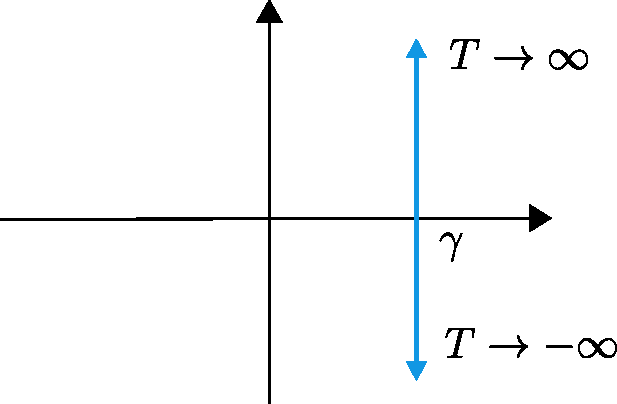
\includegraphics[width=0.5\textwidth]{figure/2026-04-30.pdf}
\caption{The blue pale thing here is the what we are integrating}
\end{figure}


